\documentclass{standalone}
\usepackage{pgfplots}
\pgfplotsset{compat=1.11}
\begin{document}
% Place the TikZ picture in a figure environment.
%\begin{figure}[htb]
% h: here, t: top, b: bottom, p: page of float
%% https://tex.stackexchange.com/questions/39017/how-to-influence-the-position-of-float-environments-like-figure-and-table-in-lat
%% ! indicates that some restrictions should be ignored (discussed later)
%% h indicates that the float is allowed to be placed inline
%% t indicates that the float is allowed to go into a top area
%% b indicates that the float is allowed to go into a bottom area
%% p indicates the the float is allowed to go on a float page or column area

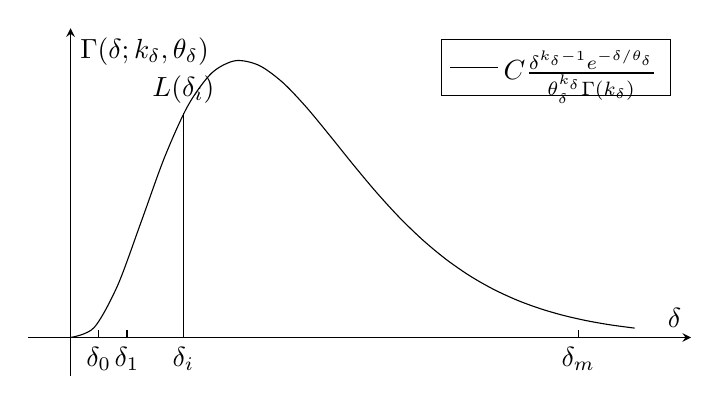
\begin{tikzpicture}[ declare function={gamma(\z)=
    (2.506628274631*sqrt(1/\z) + 0.20888568*(1/\z)^(1.5) + 0.00870357*(1/\z)^(2.5) - (174.2106599*(1/\z)^(3.5))/25920 - (715.6423511*(1/\z)^(4.5))/1244160)*exp((-ln(1/\z)-1)*\z);},
    declare function={gammapdf(\x,\k,\theta) = \x^(\k-1)*exp(-\x/\theta) / (\theta^\k*gamma(\k+1)/\k);}
]
        \begin{axis} [
        width=10cm,height=6cm,
             xmin=-1.5, xmax=22, ymin=-2.5, ymax=20,
            % xtick={-0.5,...,20}, 
            % xtick={$\delta_0$,$\delta_1$},
            % ytick={-2,-1.5,...,2},
            xticklabel style={font=\tiny, xshift=0.5ex},
            yticklabel style={font=\tiny, yshift=0.5ex},
            axis line style={->},
            axis x line=middle,
            axis y line=middle,
            ticks=none,
            xlabel={$\delta$},
            ylabel={$\Gamma(\delta; k_\delta, \theta_\delta)$},
            legend pos=north east
          % legend style={at={(0.17,0.8)},anchor=south west}
        ]
        \addplot [smooth, domain=0:20, black] {160*gammapdf(x,4,2.0)};
        \addplot[-,color=black] coordinates {(4,0) (4,14.5)};
        \node[below] (deltai) at (4,0) {$\delta_i$};
        \node[above] (Ldeltai) at (4,14.5) {$L(\delta_i)$};
        
        \node[below] (delta0) at (1, 0) {$\delta_0$};        
        \node[below] (delta1) at (2, 0) {$\delta_1$};        
        \node[below] (deltak) at (18, 0) {$\delta_m$};        

        \addplot[-,color=black] coordinates {(1,0) (1,0.5)};
        \addplot[-,color=black] coordinates {(2,0) (2,0.5)};
        \addplot[-,color=black] coordinates {(18,0) (18,0.5)};

        \addlegendentry{$C\frac{\delta^{k_\delta-1} e^{-\delta/\theta_\delta} }{\theta_\delta^{k_\delta}\Gamma(k_\delta)}$}
        \end{axis}
    \end{tikzpicture}

\end{document}